\section{ГЛАВА 5 РАЗРАБОТКА МОБИЛЬНОГО ПРИЛОЖЕНИЯ}

После определения архитектур принципов был выполнен плавный переход к разработке мобильного приложения следуя определенным нами приниципам. 
Первой частью было создание базовой структуры приложения.

\subsection*{5.1 Базовая структура приложения}
\addcontentsline{toc}{subsection}{5.1 Базовая структура приложения}
Следуя выбранному нами подходу feature-first, сначала создавалась функциональность и только внутри нее определялись слои. 
Таким образом, получилась древовидная структура, где одна функциональность могла содержать в себе другие подфункциональности, 
но благодаря продуманному делению на функциональности в проекте сложно было запутаться. 
Основной функциональностью нашего приложения, конечно, является функциональность с контентом, где мы получаем, фильтруем и создаем маршруты. 
На примере этой функциональности можно рассмотреть удобство использования feature-first подхода. На Рис.~\ref{fig:feature_structure} видно взаимосвязь функциональностей контента в мобильном приложении, а именно, что функциональность контента содержит функциональности просмотра списка маршрутов, подробной информации о конкретном маршруте, а также создания маршрута, есть общая папка, названная shared, которая содержит общий код для всех функциональностей, такой как например слой данных, общий скоуп контента и также часть общих виджетов, которые переиспользуются в нескольких функциональностях.

\begin{landscape}
\begin{figure}[H]
\centering
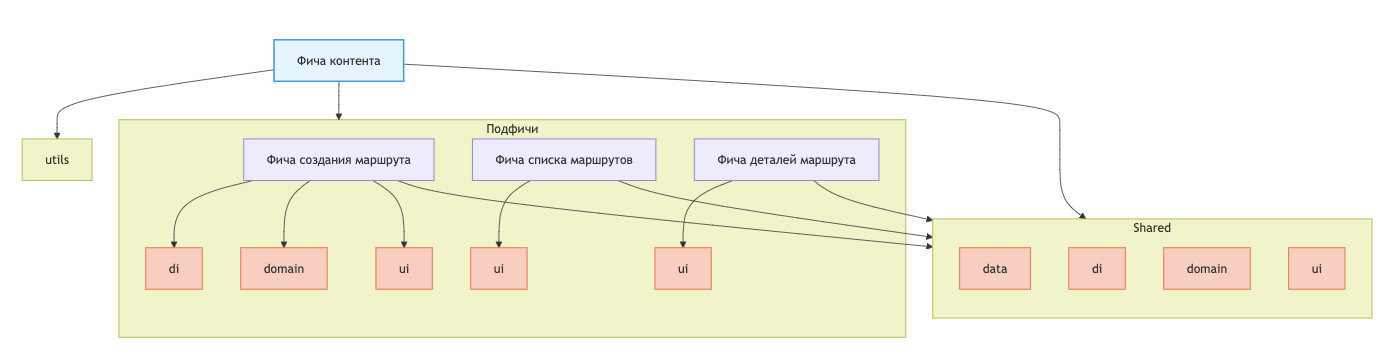
\includegraphics[height=0.4\textwidth]{Images/mobile_logic/структура_фичи.png}
\caption{Схема функциональности контента приложения}
\label{fig:feature_structure}
\end{figure}
\end{landscape}

\subsection*{5.2 Реализация слоя данных (взаимодействия с бекендом)}
\addcontentsline{toc}{subsection}{5.2 Реализация слоя данных (взаимодействия с бекендом)}
Взаимодействие с бекендом было организовано в отдельном слое - слое данных, который у каждой функциональности свой, что следует feature-first подходу. Кроме того, сами запросы отправляются через отдельные классы, которые были названы ApiClient, следуя логике, что эти классы отвечают за взаимодействие с API. А обработка исключений из этих классов была вынесены в классы, которые мы назвали, также согласно чистой архитектуре Repositories (репозиториями). Конкретную реализацию дата слоя функциональности контента можно рассмотреть на примере классов ContentApiClient и ContentApiClientImpl. Эти классы отвечают за взаимодействие с API бекенда, предоставляя методы для получения маршрутов, фильтров, загрузки изображений, а также создания мест и маршрутов. Подробный код представлен в Приложении, файл content\_api\_client.dart.

Так был создан ContentApiClient, который отвечает за взаимодействие с сервисом контента бекенда. Кроме того, следуая принципам ООП была сделана абстракция и имплементация клиента апи. Апи контента имеет 5 основных методов:

\begin{enumerate}
    \item \textbf{getRoutes} отвечает за получение списка маршрутов согласно выбранным пользователем фильтрам
    \item \textbf{getRoutesFilter} возвращает фильтров для выбора пользователем
    \item \textbf{uploadImages} позволяет загружать изображения пользователем на сервер
    \item \textbf{createPlace} отправляет запрос на создание пользвателем места маршрута
    \item \textbf{createRoute} позволяет создать маршрут
\end{enumerate}

\noindent Важно отметить, что апи слой не обрабатывает исключения, а отвечает только за передачу данных на следующий слой. Этим слоем в нашем приложении является репозиторий, а конкретно в случае функциональности контента ContentRepository и его реализация ContentRepositoryImpl. Репозиторий инкапсулирует логику получения данных от API клиента, их преобразования в модели приложения и обработку исключений. Реализацию можно увидеть в Приложении, файл content\_repository.dart.

Также была сделана абстракция репозитория, следуя принципам чистой архитектуры, также уже в репозитории происходит обработка исключений, которые может возвратить grpc. Для обработки исключений были созданы кастомные исключения, наследуемые от BaseGrpcException. Маппинг стандартных GrpcError на эти кастомные исключения происходит с помощью расширения GrpcErrorToException. Код данных исключений и расширения доступен в Приложении, файл grpc\_exceptions.dart.

Дальше полученные данные обрабатываются в соответствуюших BLoC-ах.

\subsubsection*{Получение списка маршрутов и применение фильтров}

Получение маршрута происходит через RoutesBloc. У него есть четыре состояния: RoutesLoadSuccess (успешная загрузка), RoutesInitial (начальное), RoutesLoadInProgress (загрузка) и RoutesLoadFailure (ошибка). Описание этих состояний находится в Приложении, файл routes\_state.dart.

Этот блок обрабатывает одно событие RoutesFetched, сигнализирующее о необходимости загрузить список маршрутов. Код события представлен в Приложении, файл routes\_event.dart.

Сама логика обработки события RoutesFetched и преобразования состояний происходит в RoutesBloc. Он взаимодействует с ContentRepository для получения данных. Полный код блока доступен в Приложении, файл routes\_bloc.dart.

Так как событие всего одно, то для его обработки нужен только один метод \_onGetRoutes

Для получения фильтра маршрутов был создан FilterRoutesBloc, у которого четыре состояния: FilterRoutesInitial, FilterRoutesLoadInProgress, FilterRoutesLoadSuccess (успешная загрузка доступных и пользовательских фильтров) и FilterRoutesLoadFailure. Код состояний можно найти в Приложении, файл filter\_routes\_state.dart.

Этот блок обрабатывает уже два события: AvailableFilterRoutesFetched (запрос доступных фильтров) и UserFilterRoutesChanged (изменение пользовательских фильтров). Код событий представлен в Приложении, файл filter\_routes\_event.dart.

Логика обновления состояния для FilterRoutesBloc описана в соответствующем файле. Блок обрабатывает события получения доступных фильтров и изменения пользовательских фильтров, взаимодействуя с ContentRepository. Код блока находится в Приложении, файл filter\_routes\_bloc.dart.

При этом обновление списка маршрутов происходит при изменении пользователем фильтров с помощью механизма BlocListener в виджете ContentPage. При изменении фильтров в FilterRoutesBloc, инициируется событие RoutesFetched в RoutesBloc. Код данного слушателя представлен в Приложении, файл content\_page\_listener.dart.

\subsubsection*{Создание маршрута}
Функциональность создания маршрутов является более сложной функциональностью, чем функциональности получения и фильтрацию, потому что в ней сосредоточено сразу несколько других функциональностей:

\begin{itemize}
    \item Взаимодействие с плагином Яндекс.Карт, чтобы пользователь мог выбрать точку маршрута на карте
    \item Валидация всех полей при заполнении маршрута
    \item Возможность изменять порядок мест маршрута перетаскиванием на странице создания
    \item Правильная последовательность отправки запросов на бекенд. Потому что сначала нужно отправить запрос на создание места, потом на создание фотографий и только потом создать маршрут
\end{itemize}

\noindent Для реализации этой сложной части нами было выделено 3 блока и 1 интерактор для связи этих блоков между собой.

Так как у нас есть две страницы для создания маршрута, было решено для каждой страницы сделать свой блок, чтобы перейти на следующую страницу можно было только при правильном заполнении данных на предыдущей. 

Так для  заполнения общей информации о маршруте был создан CreateRouteFormBloc. У него есть два основных состояния: CreateRouteFormEdited (форма редактируется) и CreateRouteFormFilled (форма заполнена корректно). Эти состояния содержат поля для общей информации о маршруте. Код состояний представлен в Приложении, файл create\_route\_form\_state.dart.

CreateRouteFormBloc обрабатывает события для обновления каждого поля формы (название, описание, тип транспорта и т.д.), а также событие для сброса формы. Код событий представлен в Приложении, файл create\_route\_form\_event.dart.

и сама логика обработки событий и обновления состояния определена в CreateRouteFormBloc. Блок управляет состоянием формы создания общей информации о маршруте и определяет, заполнена ли форма корректно. Полный код представлен в Приложении, файл create\_route\_form\_bloc.dart.

За создание и изменение порядка точек на маршруте отвечает CreatePointsFormBloc. У него есть одно состояние CreatePointsFormState, содержащее список моделей точек маршрута (CreatePointFormModel). Код состояния представлен в Приложении, файл create\_points\_form\_state.dart.

И этот блок обрабатывает события добавления (PlaceFormAddPoint), обновления (PlaceFormUpdatePoint), удаления (PlaceFormDeletePoint) точки, изменения порядка точек (PlaceFormReorderPoints), а также сброса формы (PlaceFormReset). Код событий представлен в Приложении, файл create\_points\_form\_event.dart.

Сама логика обновления состояния и обработки событий описана в CreatePointsFormBloc. Блок управляет списком точек маршрута. Полный код представлен в Приложении, файл create\_points\_form\_bloc.dart.

Кроме того, есть блок CreatePointFormBloc, который отвечает за редактирование точки маршрута на самой странице. Он имеет состояния для управления формой редактирования отдельной точки маршрута, такие как CreatePathPointEditedFormModel, CreatePathPointFilledFormModel, CreatePlacePointEditedFormModel, и CreatePlacePointFilledFormModel. Код состояний представлен в Приложении, файл create\_point\_form\_state.dart.

А также он содержит следующие события на изменения этого состояния. Код событий представлен в Приложении, файл create\_point\_form\_event.dart.

Сама логика обработки происходит в блоке CreatePointFormBloc. Он управляет состоянием формы редактирования отдельной точки маршрута, обрабатывает события обновления полей, управляет изображениями и определяет, заполнена ли форма точки корректно. Полный код представлен в Приложении, файл create\_point\_form\_bloc.dart.

Объединение состояния блоков CreatePointsFormBloc и CreateRouteFormBloc  происходит в методе createRoute интерактора CreateRouteInteractor. Интерактор координирует процесс создания маршрута, взаимодействуя с ContentRepository. Полный код представлен в Приложении, файл create\_route\_interactor.dart.

Для реализации функциональности создания маршрутов были выделены блоки CreateRouteFormBloc  для управления общей информацией о маршруте и CreatePointsFormBloc  для работы со списком точек маршрута, включая изменение их порядка. Отдельный блок CreatePointFormBloc  был разработан для редактирования информации по конкретной точке маршрута, учитывая различные типы точек (опорная точка или место).  

Взаимодействие между блоками CreatePointsFormBloc и CreateRouteFormBloc, а также координация отправки запросов к слою данных, реализованы в интеракторе CreateRouteInteractor, который обеспечивает правильную последовательность операций, включая создание мест и загрузку изображений перед созданием самого маршрута.  

Таким образом, в этой главе продемонстрирован подход к разработке мобильного приложения с четким разделением ответственности между компонентами с использованием BLoC и интеракторов, что способствует модульности, тестируемости и поддерживаемости кода.

\subsection*{Выводы по главе}
\addcontentsline{toc}{subsection}{Выводы по главе}
В этой главе была детально представлена практическая реализация мобильного приложения «Путешествия по России» с применением архитектурных принципов и подходов, определённых в четвёртой главе.

Успешно реализован Feature-First подход к организации кода, который продемонстрировал свою эффективность на примере функциональности контента. Древовидная структура с разделением на основные функциональности (просмотр списка маршрутов, детальная информация о маршруте, создание маршрута) и общие компоненты (shared) обеспечивает чёткую логику проекта и исключает возможность запутаться в структуре даже при масштабировании.

Реализация слоя данных продемонстрировала правильность выбора архитектурных решений. Чёткое разделение ответственности между ApiClient (взаимодействие с API) и Repository (обработка исключений и преобразование данных) обеспечивает модульность и тестируемость кода. Использование абстракций и принципов ООП позволило создать гибкую систему, легко адаптируемую под изменения требований.

Паттерн BLoC продемонстрировал свою эффективность при реализации различных по сложности функциональностей. Для простых задач (получение и фильтрация маршрутов) достаточно базовых блоков RoutesBloc и FilterRoutesBloc, тогда как для сложной функциональности создания маршрутов была успешно применена композиция из нескольких взаимодействующих блоков (CreateRouteFormBloc, CreatePointsFormBloc, CreatePointFormBloc) с координацией через интерактор CreateRouteInteractor.

Особенно важным достижением стала реализация сложной функциональности создания маршрутов, включающей интеграцию с картографическими плагинами, валидацию форм, возможность изменения порядка точек и правильную последовательность API-запросов. Применение принципа разделения ответственности позволило разбить эту задачу на управляемые компоненты без потери целостности пользовательского опыта.

Система обработки исключений с использованием кастомных исключений (AlreadyExistsGrpcException, InvalidArgumentGrpcException и др.) и их маппинга через расширения обеспечивает надёжную работу приложения и понятную обратную связь для пользователей при возникновении ошибок.

Механизм BlocListener для связи между блоками (автоматическое обновление списка маршрутов при изменении фильтров) демонстрирует элегантность реактивного подхода и его преимущества для создания отзывчивого пользовательского интерфейса.

Таким образом, в этой главе продемонстрирована практическая реализация теоретических архитектурных решений, подтверждена их эффективность и жизнеспособность. Полученная реализация обеспечивает высокое качество кода, простоту сопровождения и отличную основу для дальнейшего развития приложения.


